% IMPORTANT: PLEASE USE XeLaTeX FOR TYPESETTING
\documentclass{beamer}
\usetheme{Darmstadt}%{default}
\usecolortheme{beaver}
\usepackage[T1]{fontenc} 
\usepackage[utf8]{inputenc}
\usepackage[french]{babel}
\usefonttheme{serif}
\usepackage{lmodern}
 % pour un pdf lisible à l'écran
 % il y a d'autres choix possibles 
\usepackage{pslatex}
% \usepackage{ctex, hyperref}
\usepackage{latexsym,amsmath,xcolor,multicol,booktabs,calligra}
\usepackage{graphicx,pstricks,listings,stackengine}

% meta-data
\title{Leçon 26: Cinématique relativiste}
\subtitle{Expérience de Michelson et Morley}
\author{Gabriel Le Doudic}
\date{\today}
\institute{Préparation à l'agrégation de Rennes 1}
% \titlebackground{images/background}

% document body
\begin{document}
\maketitle
% --------- Sommaire ---------
% \begin{frame}
%     \tableofcontents
% \end{frame}      
% ----------------------------
\section{Introduction}


\section{I. Les problèmes de la cinématique classique}
\subsection{I.1. Relativité galiléenne}
\begin{frame}{I.1. Relativité galiléenne}
    \begin{columns}
        \column{.6\textwidth}
    \begin{block}{}
\begin{figure}
    \centering
    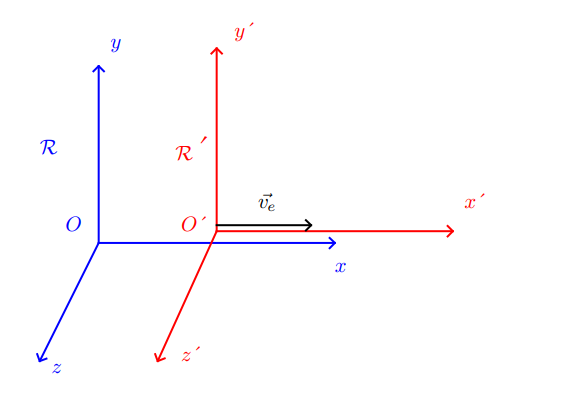
\includegraphics[width=1\textwidth]{refgalileen.png}
    \caption{Référentiel galiléen.}
\end{figure}
\end{block}
\column{.4\textwidth}
$\bullet$ Transformée de Galilée:
\begin{equation}
    \left\{\begin{array} {rcl}
        x(t) &=& x'(t) + v_e t\\
        y &=& y'\\
        z &=& z'\\
        t &=& t'\nonumber
    \end{array}\right.
\end{equation}
\end{columns}
\end{frame}

\subsection{I.2. Qu'en est-il de l'électromagnétisme ?}
\begin{frame}{I.2. Qu'en est-il de l'électromagnétisme ?}
$\bullet$ Propagation d'ondes électromagnétiques dans le vide:
\begin{equation}
    \Delta E = \dfrac{1}{c^2}\dfrac{\partial^2 E}{\partial t^2}.
\end{equation}

\begin{alertblock}{Conclusion}
    \begin{itemize}
        \item Les équations de Maxwell $\rightarrow$ ondes électromagnétiques de vitesse $c$.

    \item Si la vitesse de la lumière est définie dans un référentiel privilégié et si elle obéit à la loi decomposition des vitesses on doit pouvoir mesurer une variation de la vitesse de la lumière.
    \end{itemize}
\end{alertblock}

% \begin{block}{Remark}
%     Sample text
%     \end{block}
    
%     \begin{alertblock}{Important theorem}
%     Sample text in red box
%     \end{alertblock}
    
%     \begin{examples}
%     Sample text in green box. The title of the block is ``Examples".
%     \end{examples}
\end{frame}

\section{II. L'Expérience de Michelson et Morley}

\subsection{II.1. Dispositif}

\begin{frame}{II.1. Dispositif}
    \begin{block}{}
    \begin{figure}
        \centering
        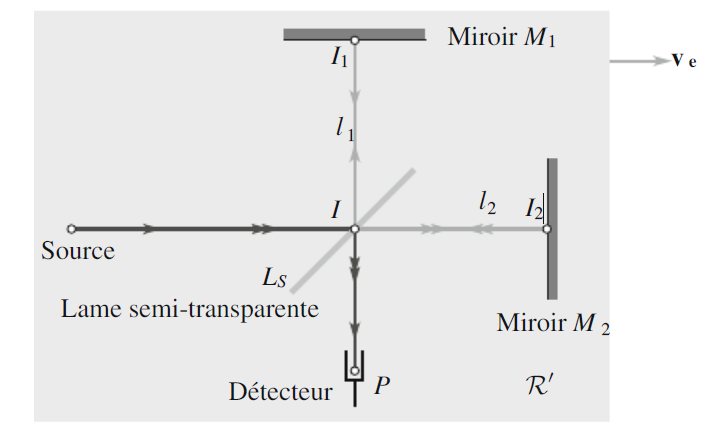
\includegraphics[width = .7\textwidth]{Michelson.png}
        \caption{Schéma de l'interféromètre de Michelson (\textit{Pérez, Relativité}).}
    \end{figure}
\end{block}
\end{frame}

\begin{frame}{II.1. Dispositif}
    \begin{columns}
        \column{0.5\textwidth}
        \begin{block}{}
            \begin{figure}
                \centering
                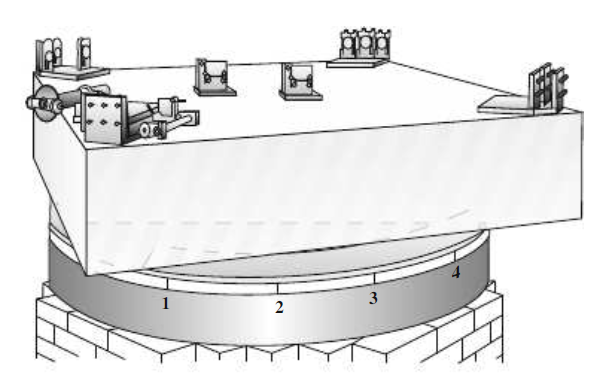
\includegraphics[width =1\textwidth]{MIchelsonMorley.png}
                \caption{Interféromètre de Michelson et Morley (\textit{Pérez, Relativité})}
            \end{figure}
        \end{block}
    \column{0.5 \textwidth}
    \begin{block}{}
        \begin{figure}
            \centering
            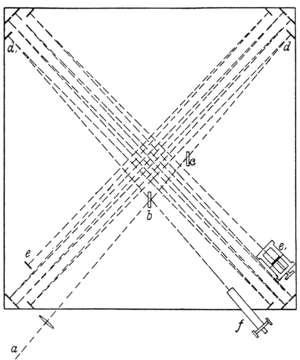
\includegraphics[width =.6\textwidth]{MIchelsonMorley2.png}
            \caption{Interféromètre de Michelson et Morley (\textit{Pérez, Relativité})}
    \end{figure}
    \end{block}
    \end{columns}
\end{frame}

\begin{frame}{II.3. Résultats}
    \begin{block}{}
        \begin{figure}
            \centering
            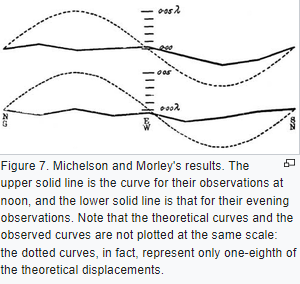
\includegraphics[width=.5\textwidth]{resultsMichelsonMorley.png}
            \caption{Résultats obtenus par Michelson et Morley (\textit{Wikipedia})}
        \end{figure}
    \end{block}
\end{frame}

\section{III.Les fondements de la relativité restreinte}
\subsection{III.1. Postulats de la relativité restreinte}
\begin{frame}{Transformée de Lorentz et composition des vitesses}
    $\bullet$ Dans le référentiel $\mathcal{R}$':
\begin{equation}
    \left\{\begin{array}{rcl}
    ct' &=& \gamma\left(ct-\beta x\right)\\
    x'&=&  \gamma\left(x'- \beta ct\right)\\
    y' &=& y\\
    z'&=& z
    \end{array}\right. \text{ avec } \left\{\begin{array}{rcl}\gamma &=&\dfrac{1}{\sqrt{1-(\dfrac{v}{c})^2}} \\ \beta &=& \dfrac{v}{c}\end{array}\right.
\end{equation}
$\bullet$ Composition des vitesses:
\begin{columns}
    \column{0.5\textwidth}
\begin{equation}
    \left\{\begin{array}{rcl}
        cdt' &=& \gamma\left(cdt-\beta dx\right)\\
        dx'&=&  \gamma\left(dx'- \beta cdt\right)\\
        dy' &=& dy\\
    \end{array}\right.
\end{equation}

\column{.5\textwidth}

\begin{equation}
    \left\{\begin{array}{rcl}
        v_x &=& \dfrac{v_x'+v_{e}}{1+v_e\dfrac{v_x'}{c^2}}\\
        v_y &=& \dfrac{v_y'}{1+v_e\dfrac{v_x'}{c^2}}
    \end{array}\right.
\end{equation}

\end{columns}

\end{frame}

\subsection{III.3. Conséquences de la relativité restreinte: Le train d'Einstein}
\begin{frame}{Le train d'Einstein}
    \vspace{-.4cm}
Consdérons un wagon de TGV de longueur $l' = 475~\rm m$ mesuré dans le référentiel lié au train $\mathcal{R}'$ qui se déplace à une vitesse $v_e=0.54c$ par rapport à un tunnel fixe dans le référentiel $\mathcal{R}$ et de longueur $L$.
\begin{columns}
    \column{0.4\textwidth}
    On relève quatre évènements différents: 
\begin{itemize}
    \item $A_1$ L'avant du train rentre dans le tunnel;
    \item $A_2$ L'avant du train sort du tunnel;
    \item $B_1$ L'arrière du train entre dans le tunnel;
    \item $B_2$ L'arrière du train sort du tunnel.
\end{itemize}
    \column{.6\textwidth}
    \begin{block}{Animation train d'Einstein}
    \begin{figure}
        \centering
        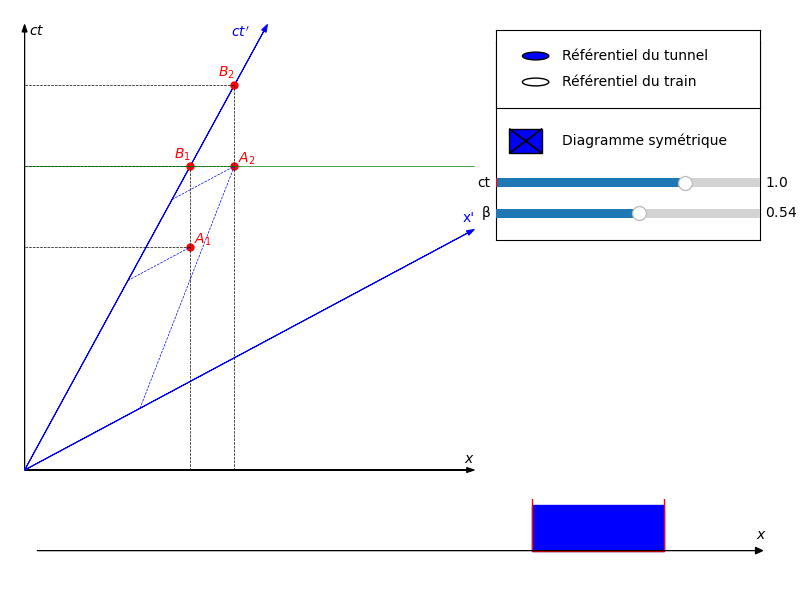
\includegraphics[width = 1\textwidth]{TrainEinstein.png}
    \end{figure}
\end{block}
\end{columns}

\end{frame}


\section{Conclusion}
\begin{frame}{Conclusion: le problème d'Einstein}
    Pour ce premier cours de relativité restreinte, nous avons établi les bases d’une nouvelle cinématique. Il faut
    maintenant établir une nouvelle dynamique. Ainsi dans un prochain cours nous mettrons en équation la dynamique
    relativiste, en particulier nous écrirons les quadrivecteurs énergie et impulsion pour une particule en mouvement.

    Affaire à suivre : 
    \begin{itemize}
        \item Quadri-vecteur impulsion : $\vec{p} = (m\gamma c, m\gamma \vec{v})$
        \item Énergie : $E^2=p^2c^2+m^2c^4$
    \end{itemize}
\end{frame} 

\end{document}